\begin{figure}[H]
    \centering
    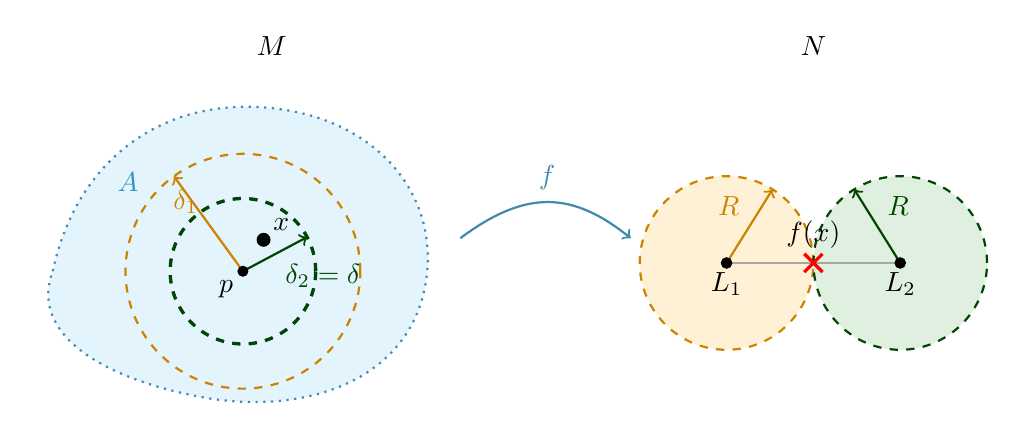
\begin{tikzpicture}[scale=1.05]
        % Dominio.
        \begin{scope}
            \node at (0,2.62) {$M$};

            \path[fill=Cerulean!11]
                (-2.65,-0.10)
                .. controls (-2.35,1.30) and (-1.25,2.05) .. (0.10,1.86)
                .. controls (1.28,1.70) and (2.04,0.82) .. (1.86,-0.25)
                .. controls (1.65,-1.45) and (0.36,-1.85) .. (-0.86,-1.62)
                .. controls (-2.04,-1.40) and (-2.94,-0.86) .. (-2.65,-0.10)
                -- cycle;
            \draw[Cerulean!72!black, thick, dotted]
                (-2.65,-0.10)
                .. controls (-2.35,1.30) and (-1.25,2.05) .. (0.10,1.86)
                .. controls (1.28,1.70) and (2.04,0.82) .. (1.86,-0.25)
                .. controls (1.65,-1.45) and (0.36,-1.85) .. (-0.86,-1.62)
                .. controls (-2.04,-1.40) and (-2.94,-0.86) .. (-2.65,-0.10)
                -- cycle;

            \coordinate (p) at (-0.35,-0.10);
            \coordinate (x) at (-0.1,0.28);

            \draw[Orange!80!black, thick, dashed] (p) circle (1.42);
            \draw[Cerulean!75!black, thick, dashed] (p) circle (0.88);
            \draw[Green!55!black, very thick, dashed] (p) circle (0.88);

            \draw[Orange!80!black, thick, ->] (p) -- ++(126:1.42)
                node[midway, above left] {$\delta_1$};
            \draw[Green!55!black, thick, ->] (p) -- ++(28:0.88)
                node[midway, below right] {$\delta_2=\delta$};

            \filldraw[black] (p) circle (1.7pt) node[below left] {$p$};
            \filldraw[black] (x) circle (2.2pt) node[above right] {$x$};
            \node[Cerulean!80!black] at (-1.74,0.98) {$A$};
        \end{scope}

        % Aplicacao.
        \draw[->, thick, Cerulean!70!black]
            (2.28,0.30) .. controls (3.06,0.88) and (3.62,0.88) .. (4.34,0.30);
        \node[Cerulean!70!black] at (3.33,1.03) {$f$};

        % Contradominio.
        \begin{scope}[xshift=6.55cm]
            \node at (0,2.62) {$N$};

            \coordinate (L1) at (-1.05,0);
            \coordinate (L2) at (1.05,0);
            \coordinate (y) at (0,0);

            \path[fill=Orange!16] (L1) circle (1.05);
            \path[fill=Green!12] (L2) circle (1.05);
            \draw[Orange!80!black, thick, dashed] (L1) circle (1.05);
            \draw[Green!55!black, thick, dashed] (L2) circle (1.05);

            \draw[gray!70, thick] (L1) -- (L2);
            \draw[Orange!80!black, thick, ->] (L1) -- ++(58:1.05)
                node[midway, above left] {$R$};
            \draw[Green!55!black, thick, ->] (L2) -- ++(122:1.05)
                node[midway, above right] {$R$};

            \filldraw[black] (L1) circle (1.8pt) node[below] {$L_1$};
            \filldraw[black] (L2) circle (1.8pt) node[below] {$L_2$};
            \draw[Red, very thick] (y) ++(-0.11,-0.11) -- ++(0.22,0.22);
            \draw[Red, very thick] (y) ++(-0.11,0.11) -- ++(0.22,-0.22);
            \node[black] at (0,0.34) {$f(x)$};
        \end{scope}
    \end{tikzpicture}
    \caption{A escolha de $\delta$ forçaria $f(x)$ a pertencer a duas bolas disjuntas.}
    \label{fig:limiteUnico}
\end{figure}
